\documentclass[11pt]{article}
\usepackage[margin=1in]{geometry}
\usepackage[T1]{fontenc}
\usepackage{lmodern}
\usepackage{microtype}
\usepackage{amsmath,amssymb}
\usepackage{booktabs,tabularx,array}
\usepackage{enumitem}
\usepackage{xcolor}
\usepackage{listings}
\usepackage{tikz}
\usetikzlibrary{arrows.meta,positioning}
\usepackage[obeyspaces,spaces]{url}
\usepackage[hidelinks]{hyperref}

\setlist{itemsep=2pt,topsep=4pt}
\setlength{\parskip}{5pt}
\setlength{\parindent}{0pt}
\setlength{\emergencystretch}{3em}
\renewcommand{\arraystretch}{1.25}
\newcolumntype{Y}{>{\raggedright\arraybackslash}X}
\newcolumntype{R}{>{\raggedleft\arraybackslash}X}

\definecolor{codebg}{RGB}{247,247,250}
\definecolor{codeframe}{RGB}{200,200,210}
\definecolor{keyword}{RGB}{30,60,140}
\definecolor{comment}{RGB}{100,110,120}
\definecolor{string}{RGB}{150,60,20}
\definecolor{notebg}{RGB}{238,244,252}
\definecolor{okbg}{RGB}{232,246,234}
\definecolor{warnbg}{RGB}{253,240,232}
\definecolor{linkc}{RGB}{20,80,170}
\definecolor{lapi}{RGB}{225,238,252}
\definecolor{leng}{RGB}{230,245,232}
\definecolor{lms4}{RGB}{252,243,224}
\definecolor{lcore}{RGB}{238,238,238}
\hypersetup{colorlinks=true,linkcolor=linkc,urlcolor=linkc,filecolor=linkc}

\lstdefinestyle{java}{language=Java, basicstyle=\ttfamily\small, columns=fullflexible, keepspaces=true,
  keywordstyle=\color{keyword}\bfseries, commentstyle=\color{comment}\itshape, stringstyle=\color{string},
  backgroundcolor=\color{codebg}, frame=single, rulecolor=\color{codeframe}, breaklines=true,
  showstringspaces=false, xleftmargin=4pt, xrightmargin=4pt, aboveskip=6pt, belowskip=6pt}
\lstset{style=java}

\newcommand{\code}[1]{\texttt{#1}}
\newcommand{\shadedbox}[3]{\par\smallskip\noindent\colorbox{#1}{\parbox{\dimexpr\linewidth-2\fboxsep}{\textbf{#2}\par #3}}\par\smallskip}
\newcommand{\takeaway}[1]{\shadedbox{okbg}{In short}{#1}}
\newcommand{\note}[1]{\shadedbox{notebg}{Note}{#1}}
\newcommand{\decision}[1]{\shadedbox{warnbg}{Decision needed}{#1}}
\newcommand{\us}{\,\textmu s}
\newcommand{\docsdir}{../}
\def\thisdoc{fastcopy}
% Shared cross-document links for the ParaDEVS documents. Each document defines \docsdir (path from its folder to
% docs/) and \thisdoc (its key below), then \input's this file.
%
% \doclink{path relative to docs/}{text}: a link to another PDF. Links are plain URI actions (file:///...), because
% Edge, Chrome and VS Code's PDF viewers ignore hyperref's usual "open another PDF" (GoToR) links. The absolute
% address comes from docroot.tex, which scripts/build_docs.sh regenerates; rerun it if the folder moves.
%
% \relateddocs: the "ParaDEVS documents" box listing every document, with the current one marked.
\InputIfFileExists{\docsdir docroot.tex}{}{\gdef\docroot{.}}
\providecommand{\thisdoc}{}
\definecolor{pdlink}{RGB}{20,80,170}
\definecolor{pdrelbg}{RGB}{243,246,252}
\definecolor{pdrelframe}{RGB}{190,200,220}
\makeatletter
\newcommand{\doclink}[2]{\hyper@linkurl{\textcolor{pdlink}{\textbf{#2}}}{\docroot/#1}}
\newcommand{\pd@item}[4]{% key, path, title, description
  \def\pd@key{#1}%
  \item \ifx\pd@key\thisdoc\textbf{#3} (this document)\else\doclink{#2}{#3}\fi: #4}
\newcommand{\relateddocs}{\par\medskip\noindent
  \fcolorbox{pdrelframe}{pdrelbg}{\parbox{\dimexpr\linewidth-2\fboxsep-2\fboxrule}{\small
  \textbf{ParaDEVS documents.} The entry point is \doclink{ParaDEVS_Start_Here.pdf}{Start Here}, a reading guide
  that links every document.
  \begin{itemize}[leftmargin=1.4em,itemsep=0pt,topsep=2pt]
  \pd@item{report}{report/ParaDEVS_Build_Report.pdf}{Build Report}{what has been built, how it was verified, what is next}
  \pd@item{howto}{howto/ParaDEVS_HowTo.pdf}{How-To Guide}{setup, tutorials, API reference, troubleshooting}
  \pd@item{architecture}{architecture/ParaDEVS_Architecture.pdf}{Architecture Guide}{how the library works and how to read results}
  \pd@item{rl}{rl/ParaDEVS_RL_Plan.pdf}{RL Plan}{reinforcement-learning plan, analysis and results}
  \pd@item{control}{rl/ParaDEVS_Control_Spec.pdf}{Control Spec}{action selection: Para.decide, graph-mode planning, value and policy iteration}
  \pd@item{hybrid}{rl/ParaDEVS_Hybrid_Study.pdf}{Hybrid Study}{which draws to enumerate or sample, and how cost grows with lookahead}
  \pd@item{fastcopy}{engine/ParaDEVS_FastCopy_Proposal.pdf}{Fast-Copy Proposal}{why the engine replays steps, where time goes, how to speed it up}
  \end{itemize}}}\par\medskip}
\makeatother


\tikzset{box/.style={draw,rounded corners=2pt,align=center,inner sep=4pt,font=\small},
  flow/.style={-{Stealth[length=2mm]},thick}, dflow/.style={-{Stealth[length=2mm]},thick,dashed},
  lbl/.style={font=\footnotesize}}

\title{\textbf{ParaDEVS Library}\\[4pt]\large Fast branch copies: a proposal for speeding up the engine}
\author{ParaDEVS Library workspace, Binghamton}
\date{October 16, 2026 \quad (proposal only: no engine code has been changed)}

\begin{document}
\maketitle

\begin{center}
\begin{minipage}{0.88\linewidth}\small
\textbf{How to read this proposal.} Page~\pageref{sec:glance} is a one-page summary. Section~\ref{sec:halfway}
answers your question about the model being ``half way through its transition''. Every later section opens with a
green ``In short'' box. Terms are defined in the glossary (Appendix~\ref{app:glossary}). Nothing in
\path{src/main} has been changed; all measurements come from a prototype in \path{src/sandbox}
(Appendix~\ref{app:repro}).
\end{minipage}
\end{center}

\relateddocs

\tableofcontents
\newpage

%=====================================================================
\section{At a glance}\label{sec:glance}

\begin{tabularx}{\linewidth}{@{}>{\bfseries\raggedright\arraybackslash}p{3.5cm}Y@{}}
\toprule
The problem & One departure (one run of one event) costs about 70--90\us{} on the FrozenLake walker and about
  250\us{} on baseball. The model's own code is only 2--5\% of that. \textbf{About 95\% is copying}: turning the saved
  bytes back into objects (70--80\%) and saving the result as bytes again (15--25\%).\\
Your question & The model cannot be reused after a draw suspends it, because it is stopped in the middle of its
  transition and Java cannot resume it. Even if it could, following $m$ outcomes needs $m$ independent copies of the
  paused run, and a paused run cannot be copied. So \emph{replaying from a clean copy is required for branching}.
  The speed-up has to come from making the copy cheap (Section~\ref{sec:halfway}).\\
What we measured & A prototype engine in \path{src/sandbox}, checked against the real engine (same values,
  departures and merges), with five ways of copying a branch.\\
Main result & Keep each finished branch as a live Java object and copy it directly in memory instead of through
  bytes: \textbf{20--25$\times$ faster on FrozenLake and 9--20$\times$ on baseball}, with no change to any model.
  A hand-written copy method (opt-in) reaches \textbf{28--35$\times$ and 29--90$\times$}.\\
Also found & (1) The merge key costs 6\% today and becomes the largest cost once copies are fast; a cheaper key
  builder fixes most of it. (2) 6--21\% of runs are thrown away (the ``discovery'' run before each draw); they can be
  avoided by letting that run continue with the first outcome. (3) Live objects use \emph{less} memory than bytes
  (MdpWalker: 280 instead of 1{,}550 bytes per branch).\\
The risk & A wrong copy gives wrong answers silently. The prototype includes a verification mode that compares every
  fast copy with a serialization copy and catches both kinds of mistake we tried, on the first copy or first run.\\
Recommendation & Phase~1 (generic fast copy, cheaper keys, verification mode in tests): about 3 days, about
  20$\times$. Phase~2 (opt-in \code{ParaCopyable}): about 1 day, a further 1.5--4$\times$ on large models.
  Phase~3 (no discovery run): about 2 days, a further 10--25\%. The 10-minute comparison study
  (\code{CompareNStep}) should drop to well under a minute.\\
\bottomrule
\end{tabularx}

\decision{Section~\ref{sec:decide} lists four points for you to decide before any engine change: whether to adopt
Phase~1 (and as the default or as an opt-in), whether to add the \code{ParaCopyable} interface to the public API,
whether Monte Carlo runs may change their random streams (Phase~3), and whether the verification mode should run in
every acceptance test.}

%=====================================================================
\section{How a departure is run today}\label{sec:today}

\takeaway{Each branch is kept as serialized bytes. Every run of an event first rebuilds the whole model from those
bytes, runs the event, and, if it finished, saves the model to bytes again. A run that reaches a draw stops, is thrown
away, and the event is re-run from the bytes once per outcome.}

The engine (\code{ParaEngine.runLocal}) does these steps for every departure:
\begin{enumerate}
\item \textbf{Restore}: \code{Snapshots.restore} deserializes the parent branch's bytes into a fresh object graph:
  the model, its ports, its MS4 simulator, and for a coupled model all children and the routing tables.
\item \textbf{Wrap}: \code{ModelNode.of} builds the small driver objects that run the model in a fixed order.
\item \textbf{Run} the event with the values supplied so far. If the model calls \code{Para.choose} for a value
  that is not supplied yet, \code{Para} throws a \code{Suspension}; MS4 wraps it in its own exception; the engine
  catches it and records the pending law. The half-run model is discarded.
\item If the event finished: fold the outputs into the observation (\textbf{record}), build the merge key
  (\textbf{key}, only with safe merging), and \textbf{save} the model to new bytes.
\end{enumerate}
So an event with one draw and $b$ outcomes is run $1+b$ times: one \emph{discovery} run that finds the law and is
thrown away, then one replay per outcome, each from a fresh restore (Figure~\ref{fig:replay}).

\begin{figure}[h]
\centering
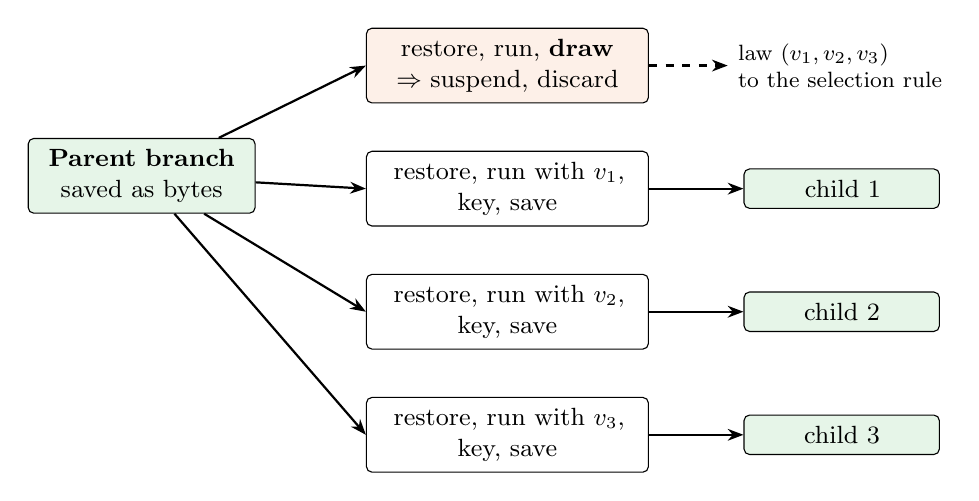
\begin{tikzpicture}[node distance=6mm and 9mm]
\node[box,fill=leng,text width=2.6cm] (p) {\textbf{Parent branch}\\saved as bytes};
\node[box,fill=warnbg,text width=3.3cm,right=14mm of p,yshift=14mm] (d) {restore, run, \textbf{draw}\\$\Rightarrow$ suspend, discard};
\node[box,text width=3.3cm,below=of d] (r1) {restore, run with $v_1$,\\key, save};
\node[box,text width=3.3cm,below=of r1] (r2) {restore, run with $v_2$,\\key, save};
\node[box,text width=3.3cm,below=of r2] (r3) {restore, run with $v_3$,\\key, save};
\node[box,fill=leng,text width=2.2cm,right=12mm of r1] (c1) {child 1};
\node[box,fill=leng,text width=2.2cm,right=12mm of r2] (c2) {child 2};
\node[box,fill=leng,text width=2.2cm,right=12mm of r3] (c3) {child 3};
\draw[flow] (p) -- (d.west); \draw[flow] (p) -- (r1.west); \draw[flow] (p) -- (r2.west); \draw[flow] (p) -- (r3.west);
\draw[flow] (r1) -- (c1); \draw[flow] (r2) -- (c2); \draw[flow] (r3) -- (c3);
\draw[dflow] (d.east) -- ++(10mm,0) node[right,lbl,align=left]{law $(v_1,v_2,v_3)$\\to the selection rule};
\end{tikzpicture}
\caption{One event with one draw and three outcomes: four runs, four restores, three saves. The first run only
discovers the law.}
\label{fig:replay}
\end{figure}

%=====================================================================
\section{Why the half-way model cannot be reused}\label{sec:halfway}

\takeaway{When a draw suspends a run, the model object is in the middle of its transition: some fields are already
updated, others are not, and part of the state lives only in Java's call stack, which the suspension destroys. Java
cannot pause a method and resume it later. Even with real pausing, branching into $m$ outcomes needs $m$ independent
copies of the paused run, and a paused run (its stack) cannot be copied. So branching must restart from a clean copy
of the state before the event. What \emph{can} be saved is the cost of that copy, and the one wasted run.}

\subsection{What ``half way through its transition'' means}
Take the moment \code{Para.choose} throws. At that moment:
\begin{itemize}
\item \textbf{The model's fields are partly updated.} A transition is ordinary Java code that assigns fields one
  after another. Everything assigned before the draw is already changed; everything after it is not. In
  \code{MdpWalker} in \code{SEPARATE} mode, the action has been drawn and the state not yet; in \code{Batter} the
  input has been read and the hit not yet chosen.
\item \textbf{MS4's bookkeeping has moved on.} Before calling the model, MS4's simulator has already set its current
  time and fired its transition event; after the call it would set the last and next event times, but that part never
  runs. In a coupled model, children earlier in the order may have finished their transitions while later ones have
  not started.
\item \textbf{Some of the state exists only on the call stack.} Local variables (the drawn action \code{a}, the row of
  probabilities, the coordinator's in-box of messages being routed) live in the stack frames of the methods that are
  running. The suspension is an exception: it unwinds the stack, and those frames are gone.
\end{itemize}
The object that is left is neither the state before the event nor the state after it. It cannot be saved as a branch
and it cannot be continued, so the engine throws it away.

\subsection{Why not pause instead of throwing?}
Java has no operation that stops a method in the middle and continues it later from the same point. There are two ways
to get something like it, and both fail for the same reason:
\begin{itemize}
\item \textbf{A thread per run}, blocked inside \code{Para.choose} until the engine supplies the value. This does pause
  the run with its stack intact.
\item \textbf{Continuations} (Java's virtual threads, ``Project Loom''): the same idea, cheaper.
\end{itemize}
Both give \emph{one} paused run. A draw with three outcomes needs \emph{three} runs that continue from that point, each
with a different value, and each changing its own copy of the model. That needs three copies of the paused run:
its stack frames \emph{and} every object they point to, including the model. Java cannot copy a thread or a
continuation (Loom continuations are one-shot by design), and copying the model objects is exactly the cost we are
trying to avoid. Copying a whole operating-system process (Unix \code{fork}) is not possible inside a JVM either.

\subsection{Consequence: replay is the right design, and the copy is what to speed up}
Replay from a clean copy is the standard way to branch a program that cannot be cloned (the paper calls it the
derandomized departure). Its extra cost is re-running the event code up to the draw, and that code is cheap: the
model's own code is 2--5\% of the time today (Table~\ref{tab:profile}). The expensive part is the copy. Hence the
proposal:
\begin{enumerate}
\item make the copy cheap (Sections~\ref{sec:generic} and~\ref{sec:hook});
\item stop paying for work that is thrown away (Section~\ref{sec:waste}). The half-way run cannot serve $m$ outcomes,
  but it can serve \emph{one}: if it simply continues with the first outcome instead of stopping, it becomes the first
  child and nothing is wasted.
\end{enumerate}

%=====================================================================
\section{Where the time goes}\label{sec:profile}

\takeaway{Restoring from bytes takes 70--80\% of a departure and saving takes 15--25\%. The model's own code takes
2--5\%. The merge key takes 6\% on baseball with merging. Runs that end at a draw (and are discarded) take 5--19\% of
the time.}

\subsection{Method}
The prototype \code{sandbox.fastcopy.ProtoEngine} is a copy of \code{ParaEngine} (without input traces and acceptors,
which these workloads do not use) with \code{System.nanoTime} timers around each step. Before any timing, the
harness checks that it gives the real engine's value, number of departures and number of merges for every strategy
(FrozenLake from six start states with and without merging; baseball with 4 and 6 plate appearances). The workloads:
\begin{center}\small
\begin{tabularx}{\linewidth}{@{}lY@{}}
\toprule
\textbf{Workload} & \textbf{What it runs}\\
\midrule
FL exhaustive & \code{MdpWalker} on FrozenLake 8$\times$8 (the $\varepsilon$-soft policy of \code{CompareNStep}),
  6-step targets from start states 0, 10, 18, 33, 44, 57, every outcome, no merging.\\
FL exhaustive + merge & The same with safe merging (repeated 8 times for stable timing).\\
FL $k{=}3$ tree + merge & Monte Carlo with 3 samples per draw and safe merging, 20 seeds per start state: the kind of
  run that dominates \code{CompareNStep}.\\
BB 5 PA & Baseball (coupled model: \code{Batter} + \code{BallGame}), 5 plate appearances, no merging.\\
BB 6 PA + merge & Baseball, 6 plate appearances, safe merging (repeated 6 times).\\
\bottomrule
\end{tabularx}
\end{center}
All runs: JDK 17.0.15, \code{-Xmx512m}, two processors, Windows 11, on a machine shared with other jobs. Single
numbers vary by about $\pm$30\% between runs; the ratios in Section~\ref{sec:results} are stable.

\subsection{Profile under today's serialization}
\begin{table}[ht]
\centering\footnotesize
\setlength{\tabcolsep}{4pt}
\begin{tabular*}{\linewidth}{@{\extracolsep{\fill}}l*{8}{r}@{}}
\toprule
\textbf{Workload} & \textbf{Total} & \textbf{Restore} & \textbf{Save} & \textbf{Model} & \textbf{Key} &
  \textbf{Other} & \textbf{Bytes} & \textbf{Susp.}\\
\midrule
FL exhaustive        & 71.9 & 57.4 (80\%) & 10.6 (15\%) & 2.4 (3\%) & 0.0 & 1.6 (2\%) & 1{,}531 & 12.7\%\\
FL exh.\ + merge     & 82.5 & 65.7 (80\%) & 11.6 (14\%) & 3.2 (4\%) & 0.3 & 1.8 (2\%) & 1{,}531 & 17.3\%\\
FL $k{=}3$ + merge   & 72.8 & 58.2 (80\%) &  9.7 (13\%) & 3.0 (4\%) & 0.2 & 1.7 (2\%) & 1{,}531 & 21.3\%\\
BB 5 PA              & 249  & 184 (74\%)  & 58.8 (24\%) & 4.1 (2\%) & 0.0 & 2.4 (1\%) & 4{,}803 &  6.5\%\\
BB 6 PA + merge      & 271  & 188 (69\%)  & 56.4 (21\%) & 4.8 (2\%) & 16.3 (6\%) & 5.6 (2\%) & 4{,}806 & 12.0\%\\
\bottomrule
\end{tabular*}
\caption{Time per departure in microseconds (share of the total in brackets). ``Model'': the event's own code,
including the throw when it suspends. ``Other'': wrapping, recording the outputs and the engine's bookkeeping.
``Bytes'': size of one saved state. ``Susp.'': share of runs that end at a draw (the discarded discovery runs).}
\label{tab:profile}
\end{table}

What this shows:
\begin{itemize}
\item \textbf{Copying is the whole cost.} The state of \code{MdpWalker} is four numbers, but its serialized form is
  1{,}531 bytes, because it includes the class descriptions of the model, its ports, its MS4 simulator and their
  lists, written out afresh in every snapshot. Reading it back means looking up each class by name and building every
  object through the serialization machinery. Baseball's snapshot (4{,}800 bytes) also carries both batting tables
  and MS4's routing tables.
\item \textbf{Restoring costs 5 times more than saving}, mostly class lookups and object construction.
\item \textbf{The discovery runs} (one per departure that draws) cost 5--19\% of the time today: 12--21\% of runs on
  FrozenLake, 6--12\% on baseball.
\item \textbf{The merge key} on baseball costs 16\us{}: \code{StateKeys} converts both batting tables into lists of
  boxed numbers on every completed departure, and recomputes field lists by reflection each time. For \code{MdpWalker}
  it is negligible because the model supplies its own key (\code{ParaStateKey}).
\item \textbf{Wrapping, recording and the engine's bookkeeping} are 1--2\% (\code{ModelNode.of} alone is under
  1\us{}). Re-creating the simulator wrappers is not worth optimizing.
\end{itemize}

%=====================================================================
\section{Option B: a generic fast copy, no model changes}\label{sec:generic}

\takeaway{Keep each finished branch as the live Java object that produced it (it is never touched again), and start
each run from an in-memory deep copy made by reflection instead of from bytes. This gives 20--25$\times$ on FrozenLake
and 9--20$\times$ on baseball, works for any model the current code supports, and falls back to serialization for
anything it does not understand.}

\subsection{The idea}
Today a finished run is saved to bytes and the object is dropped. Instead, the finished object itself can be stored as
the branch state, as long as nothing ever changes it again. Every later run of that branch starts from a copy. This
removes the save step completely and replaces ``bytes to objects'' by ``objects to objects''.

The copy (\code{sandbox.fastcopy.ReflectCopy}) visits the object graph once and produces the same graph that a
serialize-deserialize round trip produces:
\begin{itemize}
\item strings, boxed numbers, enums and classes are shared (they cannot change);
\item arrays are copied element by element;
\item JDK lists, maps, sets and priority queues are rebuilt through their normal methods, so hash tables are rebuilt
  for the new keys (MS4's routing table is a hash map keyed by port objects, so a field-by-field copy would break it);
\item every other object must be serializable without custom serialization code; it is created the way serialization
  creates it (no constructor run) and its fields are copied; fields marked \code{transient} are left empty, exactly as
  serialization leaves them;
\item what is learnt about a class (its fields, how to create it) is computed once and cached.
\end{itemize}
Anything else (a class with its own \code{readObject}, an unusual JDK collection) makes that model class fall back to
today's serialization, so no model stops working.

\subsection{A cheaper merge key}
Once copies are cheap, the merge key becomes the largest cost on baseball. The prototype \code{FastKeys} builds
\emph{exactly the same equalities} as \code{StateKeys}, but caches each class's field list, keeps a primitive array as
one wrapped copy instead of a list of boxed numbers, and caches the key's hash code so the merge table does not walk
it again. On baseball with merging this cuts the key from 16\us{} to about 4--5\us{} per departure.

\subsection{A cheaper serialization (for the fallback)}
For models that must stay on serialization, two small changes make it 1.3--1.7$\times$ faster: caching the
name-to-class lookup that deserialization does for every class description, and reusing the output buffer
(\code{SERIAL\_TUNED} in the tables). A faster third-party serializer (Kryo, FST) would add a dependency and has the
same correctness questions as the reflective copy, for less gain, so it is not proposed.

%=====================================================================
\section{Option A: an opt-in hand-written copy}\label{sec:hook}

\takeaway{A model can implement \code{ParaCopyable} and copy its own fields in a few lines; the engine copies MS4's
bookkeeping itself. Read-only data (tables) can then be shared instead of copied. This is the fastest option,
especially for coupled and larger models (baseball up to 90$\times$), but a mistake in the copy gives wrong answers,
so it needs the verification mode of Section~\ref{sec:safety}.}

\begin{lstlisting}
public interface ParaCopyable {
    /** A new, independent model with the same state. Copy only this model's own fields;
        the engine copies MS4's event times. Read-only data may be shared. */
    AtomicModel paraCopy();
}

public class FastMdpWalker extends MdpWalker implements ParaCopyable {
    @Override public AtomicModel paraCopy() {
        FastMdpWalker c = new FastMdpWalker(mdpName, startState, steps, mode);
        c.s = s; c.left = left; c.done = done; c.sigma = sigma;
        return c;
    }
}
\end{lstlisting}

The model builds a fresh instance through its normal constructor (which creates ports and the MS4 simulator) and sets
its state fields. The engine then copies the MS4 bookkeeping (the simulator's last, next and current times and its
flags) for the model and, for a coupled model, for every child in order (\code{sandbox.fastcopy.Bookkeeping}). For
baseball the copy shares the two batting tables, which never change; the generic copy has to copy them because it
cannot know that. Models that do not implement the interface use the generic copy, or serialization.

The prototype adds the hook to the two example models (\code{sandbox.fastcopy.FastModels}): 4 lines for
\code{MdpWalker}, about 15 for baseball.

%=====================================================================
\section{Option C: stop doing work that is thrown away}\label{sec:waste}

\takeaway{The discovery run before each draw is pure waste: 6--21\% of all runs. If, at a draw with no supplied value,
\code{Para} asks the engine for the options right there and lets the run continue with the first one, that run becomes
the first child and only the other outcomes are replayed. This removes every discarded run (and the exception that
MS4 builds for it) and gives a further 10--25\%, with identical results for exhaustive runs.}

\subsection{Continue with the first option}
This is how the half-way run \emph{can} be reused: not by pausing it, but by never stopping it. When \code{Para.choose}
reaches a value that has not been supplied, it calls back into the engine, which runs the selection rule, queues the
other selected values for replay (each with the values used so far), and returns the first value. The run goes on and
finishes as the first child with weight $w\alpha_1$. A second draw in the same event works the same way. An event with
one draw and $b$ outcomes is then run $b$ times instead of $b+1$.

The prototype implements it with a small addition to a \emph{copy} of \code{Para} in \path{src/sandbox/patches} (not
compiled into the library) and an \code{inline} switch in \code{ProtoEngine}. Measured:
\begin{center}\small
\begin{tabularx}{\linewidth}{@{}lRRY@{}}
\toprule
\textbf{Workload} & \textbf{Departures today} & \textbf{With inline} & \textbf{Result}\\
\midrule
FL exhaustive        & 30{,}358 & 26{,}500 ($-$13\%) & same value\\
FL exhaustive + merge (8$\times$) & 35{,}016 & 28{,}944 ($-$17\%) & same value\\
FL $k{=}3$ + merge   & 24{,}927 & 19{,}629 ($-$21\%) & statistically equivalent (different random stream)\\
BB 5 PA              & 18{,}200 & 17{,}023 ($-$6\%)  & same value\\
BB 6 PA + merge (6$\times$) & 17{,}946 & 15{,}786 ($-$12\%) & same value\\
\bottomrule
\end{tabularx}
\end{center}
The saving equals the share of runs that used to suspend. Because the selection rule is now called while the branch
is running instead of afterwards, Monte Carlo runs draw their random numbers in a different order: their results are
equally valid but not identical to today's for the same seed. Exhaustive runs give the same answers (to the last few
bits of floating-point summation order).

\subsection{The suspension exception}
MS4's simulator catches every exception from model code and wraps it in a new MS4 exception
(\code{DEVSRuntimeException}), which records a full stack trace. That costs about 1.4--1.8\us{} per suspension (a stack-less exception costs 0.03\us). It is
invisible today but becomes about 5--10\% of a departure once copies are fast. Continuing with the first option
removes suspensions altogether, so this cost disappears with it.

\subsection{Ideas measured or considered and not proposed}
\begin{itemize}
\item \textbf{Re-using the wrappers} (\code{ModelNode}): under 1\us{} per departure; not worth the complexity.
\item \textbf{Letting the last outcome run on the parent itself} instead of a copy: it saves one copy per draw, but
  if that run reaches a second draw the parent is destroyed while still needed. Unsafe in general for a small gain.
\item \textbf{Threads or continuations to pause runs}: cannot branch (Section~\ref{sec:halfway}).
\end{itemize}

%=====================================================================
\section{Measured speed-ups}\label{sec:results}

\takeaway{Wall-clock speed-ups against today's serialization, all with identical results: the generic copy with the
cheaper key gives 15--26$\times$; the hand-written copy gives 28--89$\times$; continuing with the first option adds
7--40\% on top.}

\begin{table}[h]
\centering\small
\begin{tabularx}{\linewidth}{@{}l*{7}{R}@{}}
\toprule
\textbf{Workload} & \textbf{Today (ms)} & \textbf{Tuned serial.} & \textbf{Generic copy} & \textbf{Generic + key} &
  \textbf{Hook + key} & \textbf{Hook + key + inline} & \textbf{Verify mode}\\
\midrule
FL exhaustive       & 2{,}105 & 1.7$\times$ & 25$\times$ & 24$\times$ & 35$\times$ & 41$\times$ & 0.7$\times$\\
FL exh.\ + merge    & 3{,}060 & 1.5$\times$ & 20$\times$ & 26$\times$ & 28$\times$ & 35$\times$ & 1.1$\times$\\
FL $k{=}3$ + merge  & 1{,}922 & 1.5$\times$ & 20$\times$ & 18$\times$ & 28$\times$ & 39$\times$ & 0.4$\times$\\
BB 5 PA             & 6{,}460 & 1.6$\times$ & 16$\times$ & 20$\times$ & 89$\times$ & 95$\times$ & 1.2$\times$\\
BB 6 PA + merge     & 4{,}982 & 1.3$\times$ & 9$\times$  & 15$\times$ & 29$\times$ & 33$\times$ & 1.0$\times$\\
\bottomrule
\end{tabularx}
\caption{Speed-up of the total run time over today (best of 2 runs for the serialization strategies, best of 7 for
the fast ones; timers off). ``Hook'' uses the hand-written \code{paraCopy()}; ``key'' is the cheaper key builder;
``inline'' continues with the first option. ``Verify mode'' runs the hook and checks it against serialization on
every copy (Section~\ref{sec:safety}).}
\label{tab:speedup}
\end{table}

\textbf{Time per departure after the change.} With the hand-written copy, a FrozenLake departure takes about
2--3\us{} instead of 70--90\us{}, and a baseball departure about 4--10\us{} instead of 250--280\us. What remains is
roughly a third each for the copy, the model's own code, and the key plus the engine's bookkeeping. The generic copy
costs about 1.5\us{} for \code{MdpWalker} and 13--18\us{} for baseball, because it also copies the batting tables and
rebuilds MS4's routing maps.

\textbf{Memory.} Live objects are smaller than their bytes, because the bytes repeat every class description:
\begin{center}\small
\begin{tabularx}{0.85\linewidth}{@{}lRRR@{}}
\toprule
\textbf{Stored branch state} & \textbf{Bytes (today)} & \textbf{Generic copy} & \textbf{Hand-written copy}\\
\midrule
\code{MdpWalker}    & 1{,}553 B & 281 B & 313 B\\
Baseball game       & 4{,}812 B & 3{,}682 B & 2{,}489 B\\
\bottomrule
\end{tabularx}
\end{center}

\textbf{The 10-minute comparison study.} \code{CompareNStep} runs the same walker as the FrozenLake workloads, and
nearly all its time is departures. With a 20--30$\times$ faster departure it should take roughly 20--40 seconds
instead of about 10 minutes. This is an estimate from the profile; it will be measured once Phase~1 exists.

%=====================================================================
\section{Risks and safeguards}\label{sec:safety}

\takeaway{A fast copy that misses a field, or shares something that changes, gives wrong answers without any error.
A verification mode that makes every copy twice (fast and by serialization) and compares them catches both mistakes on
the first event. It should run in every acceptance test. Live branch states must be treated as frozen, which also
makes later parallel expansion safe.}

\subsection{What can go wrong}
\begin{enumerate}
\item \textbf{An incomplete copy}: \code{paraCopy()} forgets a field. The copy starts in the wrong state. In the
  prototype, forgetting \code{left} in \code{MdpWalker} makes the walk stop at once: the 6-step return from state 55
  becomes 0.000 instead of 0.565, with 2 departures instead of 1{,}570, and \emph{no error}.
\item \textbf{A shared mutable object}: \code{paraCopy()} shares an array or list that the model later changes.
  Each copy starts correctly, but running it changes the frozen parent and every later replay of it.
\item \textbf{The generic copy and unusual classes}: a class whose serialization does something special
  (\code{readObject}, \code{readResolve}) or a JDK collection the copier does not know. The copier detects these and
  falls back to serialization; this is safe but slow.
\item \textbf{Changing a frozen state}: anything that writes to a stored branch object (a model that caches something
  in a getter, code that holds on to a model after its run) breaks every branch that shares it. Today the bytes make
  this impossible.
\item \textbf{JDK internals}: the generic copy creates objects the way serialization does, through
  \code{sun.reflect.ReflectionFactory} (module \code{jdk.unsupported}). It is available in current JDKs and used by
  many libraries, but it is not a standard API.
\end{enumerate}

\subsection{The verification mode}
Proposed as \code{ParaSpec.verifyCopies(true)}, and switchable for a whole test run with a system property, so that
\code{scripts/build\_library.sh} can run every acceptance test once with it. For each departure it:
\begin{enumerate}
\item makes the fast copy and a serialization copy of the parent, and compares them field by field over the whole
  model tree, including MS4's event times. It ignores \code{ParaStateKey}, since a hand-written key can be as
  incomplete as a hand-written copy. A difference stops the run with the model, field and both values;
\item serializes the parent before the run and again after it; if the bytes differ, the copy shared something the run
  changed, and the run stops with that message.
\end{enumerate}
In the prototype (\code{HOOK\_VERIFY}) both deliberate bugs are caught immediately:
\begin{lstlisting}[language={}]
paraCopy() is incomplete at MdpWalker: MdpWalker.left is 0 in the fast copy but 6 in the
  serialization copy
running a copy changed its parent MdpWalker: paraCopy() shares mutable state between the
  copy and the original
\end{lstlisting}
Verification costs about what today's engine costs (0.4--1.2$\times$ today's speed in Table~\ref{tab:speedup}), so it
is fine in tests but not meant for production runs. In addition, each acceptance test should compare a run with fast
copies against a run with serialization: same distribution, same departures, same merges. The prototype harness
already does this for every strategy.

\subsection{Thread safety, for a later parallel expansion}
Fast copies do not stop the engine from expanding branches in parallel later, if these rules hold:
\begin{itemize}
\item \textbf{Frozen means read-only.} A stored branch is only ever read (copied, keyed). Several threads may copy the
  same parent at once. \code{paraCopy()} must not change the object it copies.
\item \textbf{Hand-over between threads} goes through the engine's own concurrent queues, which makes the frozen
  object safely visible to the other thread.
\item \textbf{Caches are concurrent.} The copier's class plans, the key builder's field lists and the class-lookup
  cache are concurrent maps holding data that never changes once computed.
\item \textbf{Draw context}: \code{Para}'s context is already per thread. The selection rule's random generator is
  shared today; a parallel engine needs one generator per branch (split from the seed) to stay reproducible.
\item \textbf{Constructors in \code{paraCopy()}} run model and MS4 constructor code, which might touch static state
  (MS4's coupling class has a static field). This needs checking before parallel use. The generic copy runs no
  constructors.
\end{itemize}

%=====================================================================
\section{Recommendation}\label{sec:recommend}

\takeaway{Do Phase~1 first: it needs no model changes and gives about 20$\times$. Add the opt-in hook and the
first-option change afterwards, each on its own, with the verification mode in the tests from the start.}

\begin{center}\small
\begin{tabularx}{\linewidth}{@{}>{\raggedright\arraybackslash}p{3.2cm}Y>{\raggedright\arraybackslash}p{1.5cm}>{\raggedright\arraybackslash}p{3.1cm}@{}}
\toprule
\textbf{Phase} & \textbf{What changes} & \textbf{Effort} & \textbf{Expected gain}\\
\midrule
1. Generic fast copy & Branches hold frozen live objects; runs start from the reflective copy, with serialization as
  fallback (and the class-lookup cache for it); cheaper merge key in \code{StateKeys}; verification mode and
  fast-versus-serialization comparison in every acceptance test; architecture guide updated. &
  about 3 days & 15--25$\times$ on these models; \code{CompareNStep} from about 10 min to under a minute\\
2. \code{ParaCopyable} (opt-in) & Public interface plus engine support and MS4 bookkeeping copy; hooks on
  \code{MdpWalker} and baseball; a how-to section on writing a correct copy. & about 1 day &
  a further 1.5$\times$ (FrozenLake) to 4$\times$ (baseball)\\
3. Continue with the first option & \code{Para} asks the engine for options at an unsupplied draw; the expansion
  loop replays only the other options. & about 2 days & a further 10--25\%; removes all suspensions\\
Quick win (any time) & Only the class-lookup cache and buffer reuse in \code{Snapshots}. & 1--2 hours & 1.3--1.7$\times$\\
\bottomrule
\end{tabularx}
\end{center}

Every phase keeps today's results: exhaustive answers, departures and merges stay the same (Phase~3 changes the
departure count, by design, and the Monte Carlo random stream). All 99 checks would be re-run after each phase, plus
the same checks with verification switched on.

%=====================================================================
\section{What you need to decide}\label{sec:decide}

\takeaway{Four choices, each with a recommended answer.}

\begin{enumerate}
\item \textbf{Adopt Phase~1, and make it the default?} Recommended: yes, as the default, with serialization still
  used automatically for models the copier cannot handle and a switch to force serialization. It relies on
  \code{sun.reflect.ReflectionFactory} (Section~\ref{sec:safety}, item~5). The alternative is to require a no-argument
  constructor in every class of a model, which MS4-generated code does not always have.
\item \textbf{Add \code{ParaCopyable} to the public API?} Recommended: yes, as an opt-in for models where speed
  matters, documented together with the verification mode. It is the only option that puts correctness in the model
  author's hands.
\item \textbf{Accept a new Monte Carlo random stream (Phase~3)?} After Phase~3, a Monte Carlo run with a given seed
  gives a different, equally valid sample than today. Re-running the RL studies would then change their numbers within
  their error bars. Recommended: yes, and record it in the decision log.
\item \textbf{Run the verification mode in every acceptance test?} Recommended: yes. It roughly doubles the test time
  (a few minutes).
\end{enumerate}

\appendix
%=====================================================================
\section{Reproducing the measurements}\label{app:repro}
Everything is in \path{src/sandbox/java/sandbox/} and marked as a measurement prototype; nothing in \path{src/main}
uses it. From the repository root in Git Bash, after \code{bash scripts/build\_library.sh}:
\begin{lstlisting}[language={}]
javac -cp "build/library/classes;lib/ms4-core.jar" -d build/proto-patch \
      src/sandbox/patches/paradevs/Para.java       # only for the "inline" rows
java -Xmx512m -XX:ActiveProcessorCount=2 \
     -cp "build/proto-patch;build/library/classes;lib/ms4-core.jar" sandbox.ProfileEngine
\end{lstlisting}
Options: \code{-Dparts=123456} selects the parts (1 cross-check, 2 profiles, 3 speed-ups, 4 verification demo,
5 exception cost, 6 memory); \code{-Dwork=FL} or \code{-Dwork=BB} restricts the workloads; \code{-Dreps=2} sets the
repetitions. Each part runs in under 3 minutes. Without \path{build/proto-patch} on the class path the inline rows
are skipped.

\begin{center}\small
\begin{tabularx}{\linewidth}{@{}>{\raggedright}p{5.6cm}Y@{}}
\toprule
\textbf{File (in \path{src/sandbox/})} & \textbf{Contents}\\
\midrule
\path{java/sandbox/ProfileEngine.java} & The harness: workloads, cross-check with the real engine, tables, demos\\
\path{java/sandbox/fastcopy/ProtoEngine.java} & Instrumented copy of the engine with the copy strategies\\
\path{java/sandbox/fastcopy/ReflectCopy.java} & Generic reflective deep copy (Option B)\\
\path{java/sandbox/fastcopy/FastKeys.java} & Cheaper merge key with the same equalities\\
\path{java/sandbox/fastcopy/ParaCopyable.java}, \path{Bookkeeping.java} & The opt-in hook and the MS4 bookkeeping
  copy (Option A)\\
\path{java/sandbox/fastcopy/FastModels.java} & Example models with \code{paraCopy()}, plus two deliberately wrong
  copies\\
\path{java/sandbox/fastcopy/Verify.java} & The verification check\\
\path{patches/paradevs/Para.java} & Copy of \code{Para} with the ``continue with the first option'' call-back (not
  compiled by the build)\\
\bottomrule
\end{tabularx}
\end{center}

%=====================================================================
\section{Glossary}\label{app:glossary}
\begin{tabularx}{\linewidth}{@{}>{\bfseries}p{3.6cm}Y@{}}
\toprule
Departure & One run of one event from a saved branch state; the unit counted in the run statistics.\\
Draw & One call to \code{Para.choose}: a random value with a known finite law.\\
Suspension & What happens when a draw's value is not yet supplied: \code{Para} throws, the run stops, and the engine
  learns the law.\\
Discovery run & The first run of an event, which only finds out the law of its first draw and is then discarded.\\
Replay & Running the event again from the parent's saved state, with the drawn values supplied.\\
Branch state & The saved model state of a branch. Today: serialized bytes. Proposed: a frozen live object.\\
Serialization & Java's built-in way of turning an object graph into bytes (save) and back (restore).\\
Deep copy & A copy of an object together with everything it refers to, so that changing one never affects the other.\\
Aliased object & An object referred to by both the original and the copy; harmless if it never changes,
  a silent bug if it does.\\
Reflection & Java's ability to read and write an object's fields by name at run time.\\
Frozen & A stored branch object that nobody changes any more; it is only copied and read.\\
\code{ParaCopyable} & Proposed opt-in interface: the model copies its own fields in \code{paraCopy()}.\\
MS4 bookkeeping & The event times and flags kept by MS4's simulator for each atomic model.\\
Merge key & The value \code{StateKeys} builds from a model's complete state; equal keys may be merged safely.\\
Continue with the first option & Proposed change: at an unsupplied draw, the run goes on with the first selected
  value instead of stopping, and only the other values are replayed.\\
Continuation / virtual thread & Java mechanisms that pause a running method; they cannot be copied, so they cannot
  branch.\\
Verification mode & Test setting in which every fast copy is checked against a serialization copy.\\
\textmu s & Microsecond, a millionth of a second.\\
\bottomrule
\end{tabularx}

\end{document}
